\subsection{State-of-the-Art Approach}
We consider model parallelism to accelerate the training of DNN on a
distributed-memory system using MPI. Figure~\ref{fig:altsplit_baseline}
illustrates the state-of-the-art approach to it which also serves as the baseline of
this chapter. It depicts a 5-hidden-layer all-connected DNN split on two MPI
processes and the 4 neurons per layer are evenly assigned to each MPI
process. The input and output layer are omitted and we assume they are
replicated in every MPI process. The black arrows in the figure indicate
all-to-all communications between the two MPI processes. During both the
forward- and backward-propagation, each neuron from the current layer needs
the outputs of the entire neurons from the preceding layer. All-to-all
communication must be performed across all the MPI processes. In the figure,
prior to the computation of each layer 4 all-to-all communication need to
occur so that the output information from the preceding layer can get to be
fully propagated to the respective portions of the current layer to all the
MPI processes. Albeit some numerical rounding errors introduced due to the
non-deterministic nature of the all-to-all communication, this approach
guarantees that the output information from the preceding layer is consistent
and identical to all the MPI processes prior to the computation of their
respective portions of the current layer.
\begin{figure}[H]
    \centerline{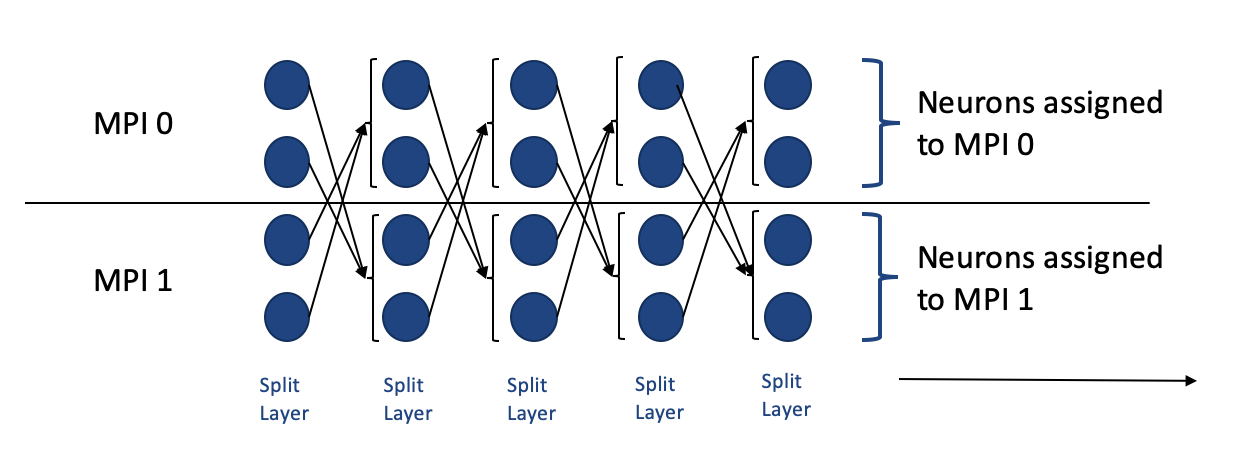
\includegraphics[scale=0.60]{altsplit/figs/baseline.png}}
    \caption{State-of-the-art model parallelism scheme}
    \label{fig:altsplit_baseline}
\end{figure}

We first show the sequential training of a DNN using matrix operations in 
Algorithm~\ref{alg:altsplit_sequential}. We denote $bs$ as the batch size, $L$ 
as the number of layers and $N_l$ as the number of neurons in layer $l$. Matrix 
of layer $l$ is denoted as $\pmb{A}_l[m,n]$ whereas $m$ and $n$ stand for the 
number of rows and columns respectively of the matrix and $(\pmb{A}_l)^T[m,n]$ 
denotes the transpose of the matrix $\pmb{A}_l$ and [m,n] represents the 
dimension of the transposed matrix.  $\nabla \pmb{A}_l[m,n]$ represents the 
gradients of matrix $\pmb{A}_l$. $\phi$ is an element-wise non-linear function 
(tanh, relu etc.). Only the operations on the forward- and backward-propagation 
phases for the hidden layers are shown in detail since they are the regions of 
interest with regard to the subsequent parallel versions of the algorithm.
\begin{algorithm}[H]%algorithm* occupies full page
\caption{Sequential DNN}
\label{alg:altsplit_sequential}
{\fontsize{10}{10}\selectfont
\begin{algorithmic}[1]
    \For {$l = 1 \ldots L$}
    \Comment Forward-propagation \State $\pmb{Y}_l[bs, N_l] = \pmb{O}_{l-1}[bs, N_{l-1}] * (\pmb{W}_{l})^T[N_{l-1}, N_l]$
        \State $\pmb{O}_l[bs, N_l] = \phi(\pmb{Y}[bs, N_l])$
    \EndFor
    \For {$l = L \ldots 1$}
    \Comment Backpropagation 
        \State $\nabla \pmb{W}_l[bs, N_l]  = \nabla \pmb{W}_{l+1}[bs, N_{l+1}] * \pmb{W}_{l+1}[N_{l+1}, N_l]$
        \State $\nabla \pmb{W}_l[bs, N_l] = \nabla \pmb{W}_l[bs, N_l] * (\partial \pmb{O}_l[bs, N_l] / \partial \pmb{Y}_l[bs, N_l]$)
    \EndFor
    \State Update parameters
\end{algorithmic}}
\end{algorithm}

The state-of-the-art model parallelism of a DNN is shown in 
Algorithm~\ref{alg:altsplit_baseline}. Besides the notations we introduced in 
Algorithm~\ref{alg:altsplit_sequential}, we give some additional notations due 
to the introduction of parallelism. $size$ denotes the number of MPI processes, 
$rank$ denotes the ID of the current MPI process and $N_l$ represents the number 
of neurons assigned to each MPI process which is equivalent to 
$N_{l\_total}/size$ (here we assume that $N_{l\_total}/size$ is divisible). This 
algorithm allocates some extra space for holding the information gathered across 
all the MPI threads: 
\begin{itemize}
    \item The weight matrix of each hidden layer $\pmb{W}_l$ should be of dimension 
        $[N_l, N_{l-1}*size]$.
    \item An extra matrix to store the outputs from the preceding hidden layer 
        from all the MPI threads $\pmb{O}_{l-1}[bs, N_{l-1}*size]$.
    \item An extra matrix to store the gradients of the succeeding layer from all 
        the MPI threads $\nabla \pmb{W}_l[bs, N_l*size]$.
\end{itemize}
At the beginning of the forward-propagation phase of each hidden layer an 
\textit{MPI\_Allgather} precedes the computation to gather outputs from all 
local portions from the preceding layer. Subsequently, each MPI thread needs to 
perform a MPI\_Allreduce with the $sum$ operation on $\nabla \pmb{W}_l[bs, 
N_l*size]$ and extract its respective gradients from it during the 
backpropagation phase.

\begin{algorithm}[H]
\caption{State-of-the-art approach to model parallelism of DNN}
\label{alg:altsplit_baseline}
{\fontsize{10}{10}\selectfont
\begin{algorithmic}[1]
    \ForAll {$p \in MPI\_Processes$}
    \Comment Forward-propagation 
        \For {$l = 1 \ldots L$}
            \State MPI\_Allgather on $\pmb{O}_{l-1}[bs, N_{l-1}*size]$ from all local $\pmb{O}_{l-1}[bs, N_{l-1}]$
            \State $\pmb{Y}_l[bs, N_l] = \pmb{O}_{l-1}[bs, N_{l-1}*size] * (\pmb{W}_{l})^T[N_{l-1}*size, N_l]$
            \State $\pmb{O}_l[bs, N_l] = \phi(\pmb{Y}[bs, N_l])$
        \EndFor
    \EndFor
    \ForAll {$p \in MPI\_Processes$}
    \Comment Backpropagation 
        \For {$l = L \ldots 1$}
            \State $\nabla \pmb{W}_l[bs, N_l*size]  = \nabla \pmb{W}_{l+1}[bs, N_{l+1}] * \pmb{W}_{l+1}[N_{l+1}, N_l*size]$
            \State MPI\_Allreduce\_sum on  $\nabla \pmb{W}_l[bs, N_l*size]$
            \State Extract $\nabla \pmb{W}_{l,p}[bs, N_l]$ from $\nabla \pmb{W}_l[bs, N_l*size]$ according to $rank$
            \State $\nabla \pmb{W}_{l,p}[bs, N_l] = \nabla \pmb{W}_{l,p}[bs, N_l] * (\partial \pmb{O}_{l,p}[bs, N_l] / \partial \pmb{Y}_{l,p}[bs, N_l]$)
        \EndFor
    \EndFor
    \ForAll {$p \in MPI\_Processes$}
        \State Update parameters
    \EndFor
\end{algorithmic}}
\end{algorithm}

\subsection{The Altsplit (Alternate Split) Approach}
We propose the \emph{Altsplit} approach which splits or replicates the layers 
alternately. The scheme is illustrated in Figure~\ref{fig:altsplit_scheme} with 
the same 5-hidden-layer DNN as in Figure~\ref{fig:altsplit_baseline}. The first 
hidden layer is split across MPI processes whereas the next layer is replicated 
on the MPI processes with the same initialization values. Subsequent layers are 
constructed with alternating splits and replications. Therefore, we cut the 
amount of communication by half during the entire training compared to the 
\emph{state-of-the-art} approach by triggering communication every other layer while at 
the cost of replicating layers on each MPI process. As a consequence, the floating
point computation is increased by 25\% (twice every other layer).
\begin{figure}[H]
    \centerline{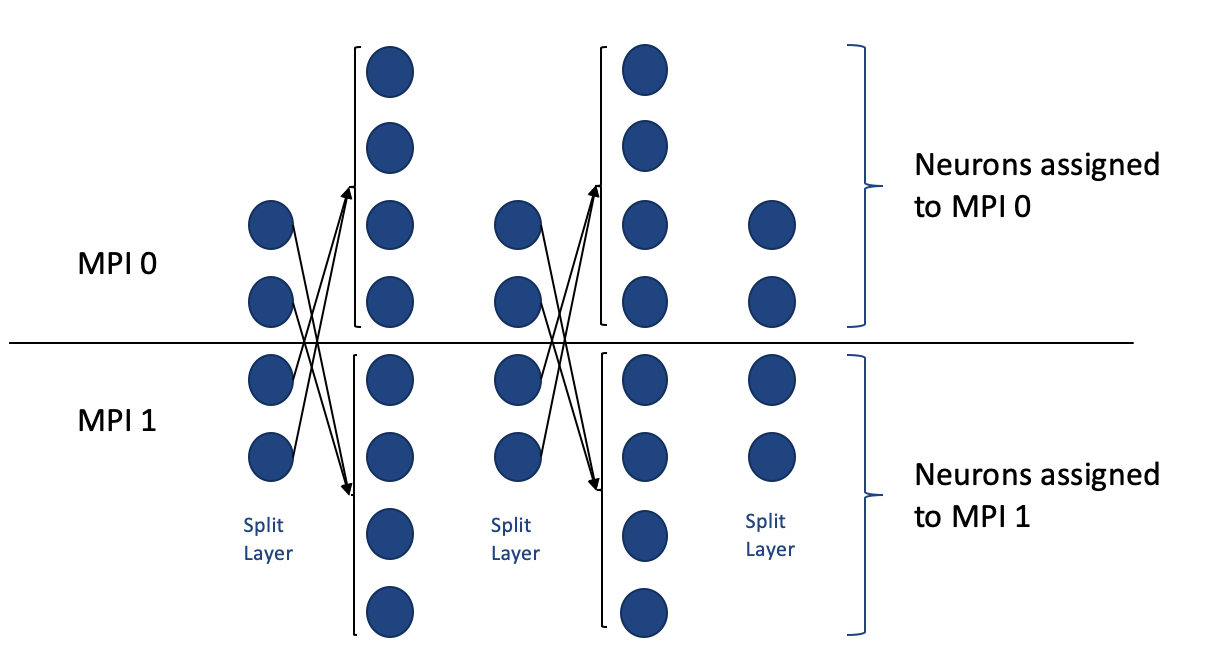
\includegraphics[scale=0.60]{altsplit/figs/altsplit.png}}
    \caption{The \emph{Altsplit} scheme}
    \label{fig:altsplit_scheme}
\end{figure}

Algorithm~\ref{alg:altsplit_altsplit} illustrates the \emph{Altsplit} approach 
to model parallelism. Unlike the state-of-the-art approach, there is no need for extra 
storage in \emph{Altsplit}. If the preceding layer during the 
forward-propagation phase is a split, an MPI\_Allreduce with the \textit{sum} 
operation must be performed on $\pmb{Y}_{l-1}[bs, N_{l}]$. Similarly, the same 
routine must be called upon on $\nabla \pmb{W}_l[bs, N_l]$ while in the 
backpropagation phase if the succeeding layer is a split.

\begin{algorithm}[H]
\caption{\emph{Altsplit} approach to model parallelism of DNN}
\label{alg:altsplit_altsplit}
{\fontsize{10}{10}\selectfont
\begin{algorithmic}[1]
    \ForAll {$p \in MPI\_Processes$}
    \Comment Forward-propagation \For {$l = 1 \ldots L$}
            \State $\pmb{Y}_l[bs, N_l] = \pmb{O}_{l-1}[bs, N_{l-1}] * (\pmb{W}_{l})^T[N_{l-1}, N_l]$
            \If {$l-1 == SPLIT$}
                \State MPI\_Allreduce\_sum on $\pmb{Y}_{l-1}[bs, N_{l}]$ 
            \EndIf
            \State $\pmb{O}_l[bs, N_l] = \phi(\pmb{Y}[bs, N_l])$
        \EndFor
    \EndFor
    \ForAll {$p \in MPI\_Processes$}
    \Comment Backpropagation \For {$l = L \ldots 1$}
            \State $\nabla \pmb{W}_l[bs, N_l]  = \nabla \pmb{W}_{l+1}[bs, 
            N_{l+1}] * \pmb{W}_{l+1}[N_{l+1}, N_l]$
            \If {$l+1 == SPLIT$}
                \State MPI\_Allreduce\_sum on $\nabla \pmb{W}_l[bs, N_l]$
            \EndIf
            \State $\nabla \pmb{W}_{l,p}[bs, N_l] = \nabla \pmb{W}_{l,p}[bs, N_l] * (\partial \pmb{O}_{l,p}[bs, N_l] / \partial \pmb{Y}_{l,p}[bs, N_l]$)
        \EndFor
    \EndFor
    \ForAll {$p \in MPI\_Processes$}
        \State Update parameters
    \EndFor
\end{algorithmic}}
\end{algorithm}
